\documentclass[12pt]{article}
% Francais UTF8
\usepackage[french]{babel}
\usepackage[utf8]{inputenc}
\usepackage[T1]{fontenc}
\usepackage{lmodern}
\usepackage{graphicx}
\usepackage[small]{caption}
\usepackage{amsmath, amssymb}
\newcommand{\R}{\mathbb{R}}
\newcommand{\Z}{\mathbb{Z}}

\newtheorem{theorem}{Théorème}
\newtheorem{definition}{Définition}

\begin{document}
\author{Gaspard Jankowiak \quad Antoine Levitt\\ Tuteur : Antoine Girard}
\title{Modèles de création d'opinion dans des réseaux sociaux}
\maketitle
\abstract{Bonjour}
\tableofcontents
\newpage
\section{Introduction}
\section{Modèles de communautés}
\subsection{Définitions}
Dans toute la suite, $(E, V)$ désigne un graphe à $n$ n\oe uds et $m$
arêtes non orienté : les éléments de $V$ sont des ensembles à deux
éléments de $E$. Ce graphe représente un réseau de $n$ individus, liés
par des relations spécifiques au domaine d'intérêt. Par exemple, on
peut prendre pour $E$ les individus d'un réseau social en ligne (type
Facebook, Myspace ...), et pour $V$ leurs relations d'amitié : $\{i, j\}
\in V$ ssi les individus $i$ et $j$ sont amis. À chaque individu $i$
on associe une valeur réelle $x_i$ représentant son opinion : l'état
du système est donc représenté par un vecteur $x \in \R^n$. On va
s'intéresser à l'évolution de cet état dans le temps dans différents
modèles.

Tout d'abord, quelques rappels de théorie des graphes. On note $d_i$
le degré du noeud $i$, égal au nombre d'arêtes incidentes au noeud $i$
: $d_i = card \{v \in V | i \in v\}$. À cette notion est associée
  celle de matrice des degrés $D$, matrice diagonale de taille $n
  \times n$ telle que $D_{i i} = d_i$. On définit également la matrice
  d'incidence $A$ telle que $A_{i j} = 1$ si $\{i, \} \in V$, $0$
  sinon.

\subsection{Graphes utilisés}
On utilise principalement deux graphes, représentés figure
\ref{graphes}.  Le premier est le réseau d'amitié dans un club de
karaté d'une université américaine dans les années 70, contenant 34
membres \cite{zachary}. Le second est le graphe d'interactions d'une
communauté de 62 dauphins \cite{dolphins}.

\begin{figure}[htb]
\centering
(a)
\includegraphics[width=.4 \textwidth]{zachary}
(b)
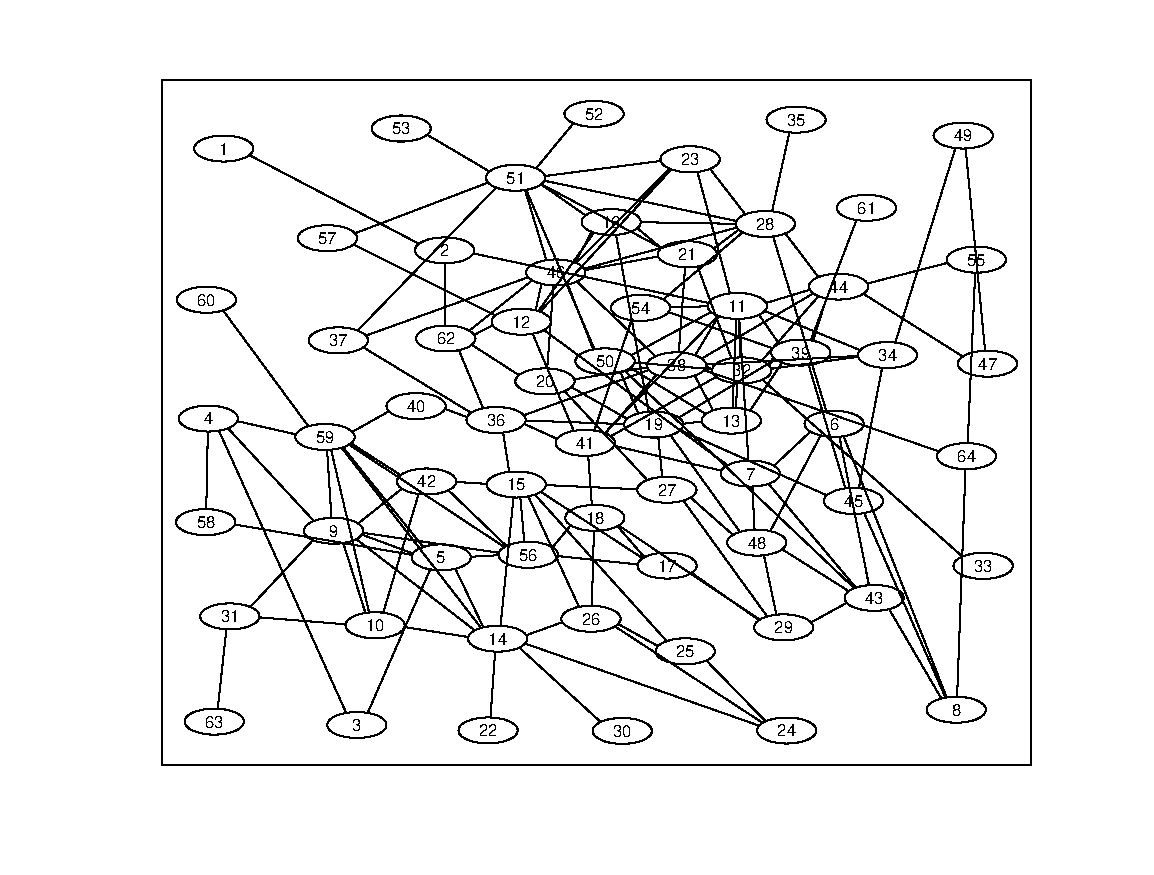
\includegraphics[width=.4 \textwidth]{dolphins}
\caption{Club de karaté de Zachary (a), et communauté de dauphins (b).}
\label{graphes}
\end{figure}

Ces graphes ont été choisis parce 
\section{Analyse spectrale de graphes et partitionnement}

\begin{thebibliography}{2}
\bibitem{zachary} W. W. Zachary, An information flow model for conflict and fission in small groups, Journal of Anthropological Research 33, 452-473 (1977)
\bibitem{dolphins} D. Lusseau, K. Schneider, O. J. Boisseau, P. Haase, E. Slooten, and S. M. Dawson, Behavioral Ecology and Sociobiology 54, 396-405 (2003)
\end{thebibliography}
\end{document}
